\documentclass[a4paper]{article}

%% Language and font encodings
\usepackage[english]{babel}
\usepackage[utf8x]{inputenc}
\usepackage[T1]{fontenc}

%% Sets page size and margins
\usepackage[a4paper,top=3cm,bottom=2cm,left=3cm,right=3cm,marginparwidth=1.75cm]{geometry}

%% Useful packages
\usepackage{amsmath}
\usepackage{graphicx}
\usepackage[colorinlistoftodos]{todonotes}
\usepackage[colorlinks=true, allcolors=blue]{hyperref}

\title{Matrici}
\author{Berlanda Federico}

\begin{document}
\maketitle

\section{Introduzione}

La matematica è il linguaggio con cui la fisica si esprime, ogni teorema e ogni legge sono enunciati attraverso i simboli che i matematici hanno creato.
\\Classicamente la branca della matematica di cui si avvalevano i fisici era l’analisi. Il grande padre della fisica, Isaac Newton, prima di creare le sue leggi, riformula le nozioni matematiche del tempo introducendo concetti rivoluzionari nel campo dell’analisi. Anche la cinematica, la termologia e l’elettromagnetismo sono teorie che si basano su questa matematica.
\\Negli ultimi anni dell’Ottocento e nei primi del Novecento la fisica attraversa un grande momento di rinnovamento e compaiono teorie rivoluzionare capaci di cambiarla per sempre. Nasce l’idea di quanto con Max Planck, poi la relatività di Eistein e la meccanica matriciale di Heisenberg e Born.
\\La grande intuizione di quest’ultimi è quella di cambiare radicalmente il punto di vista da cui si guarda il mondo della fisica; infatti quella che viene sviluppata sull’isola di Helgoland è una fisica che sfrutta un linguaggio diverso: l’algebra lineare. I due fisici tedeschi fondano la loro teoria sulle matrici, per questa ragione viene chiamata “meccanica matriciale.
\\
\\Concludo questa breve introduzione dicendo che personalmente trovo molto affascinante che un gruppo di numeri all'apparenza disposti quasi casualmente siano in grado di descrivere con tanta cura la realtà. Il mistero diventa ancora più interessante se si considera il fatto che teorie fisiche sfruttano matrici che coinvolgono numeri immaginari ottenendo risultati ottimi (un esempio sono le matrici che Pauli sfrutta per completare il suo “principio di sovrapposizione”).

\section{Le matrici}

\subsection{Presentazione del lavoro}
Quello che intendo presentare è un primo approccio all’algebra lineare e in particolare alle matrici, partendo dal definire cosa sia una matrice e illustrando le proprietà più semplici. Per questa parte della tesina faccio riferimento a tre lezioni tenute durante l’anno dal professor Bonancina e al testo {\it Matrici} della collana Schaum di Frank Ayres.

\subsection{Definizione}

\vspace*{\fill} 
\begin{quote} 
\centering 
Una matrice è una successione di numeri disposti in colonna e in riga:
\bigskip \\
$\left[\begin{matrix}a_{11} & a_{12} & ... & a_{1n} \\ a_{21} & a{22} & ... & a_{2n} \\ ... & ... & ... & ...\\ a_{m1} & a_{m2} & ... & a_{mn}\end{matrix}\right]
$
\end{quote}
\vspace*{\fill}

\section{Operazioni}
Nell'insieme delle matrici vengono definite le operazioni di somma e moltiplicazione.

\subsection{Somma}
La somma può essere effettuata solo da matrice conformabili per addizione, ovvero dello stesso ordine con ugual numero di colonne e righe. La matrice risultate avrà lo stesso ordine di quelle sommate e per ogni posizione la somma degli elementi presenti in quella posizione nelle matrici di partenza. Come esemplifica la seguente immagine:
\\
\begin{quote} \centering $\left[\begin{matrix}2 & 4 \\ 1 & 3\end{matrix}\right] + \left[\begin{matrix}5 & 3 \\ 2 & 6\end{matrix}\right] = \left[\begin{matrix} 2+5 & 4+3 \\ 1+2 & 3+6\end{matrix}\right] = \left[\begin{matrix}7 & 7 \\ 3 & 9\end{matrix}\right]
$\end{quote}

\subsubsection{Proprietà}
Questa funzione gode di queste proprietà:
\begin{itemize}
\item Commutativa, $A + B = B + A$
\item Associativa, $A + (B + C) = (A + B) + C$
\item La funzione è interna al sottoinsieme delle matrici con ordine pari a quello delle sommate.
\end{itemize}

\subsubsection{Elemento neutro}
Esiste la matrice che fra da elemento neutro, la matrice zero: 
\\
\begin{quote} \centering $\left[\begin{matrix}2 & 4 \\ 1 & 3\end{matrix}\right] + \left[\begin{matrix}0 & 0 \\ 0 & 0\end{matrix}\right] = \left[\begin{matrix}2 & 4 \\ 1 & 3\end{matrix}\right]
$\end{quote}

\subsection{Moltiplicazione}
Il prodotto fra due matrici è definito solo se le due matrici sono conformabili per la moltiplicazione, ovvero quando il numero di colonne della prima matrice è uguale al numero di righe della seconda. Il prodotto procede riga per colonna: ogni elemento della riga viene moltiplicato per il corrispondete elemento della colonna, sommando poi i prodotti.
\\
\begin{quote} \centering $\left[\begin{matrix} 2 & 3 & 4\end{matrix}\right] * \left[\begin{matrix}1 \\ -1 \\ 2 \end{matrix}\right] = \left[\begin{matrix}2*1 + 3*(-1) + 4*2 \end{matrix}\right]= \left[\begin{matrix}7\end{matrix}\right]
$\end{quote}
\begin{quote} \centering $\left[\begin{matrix} 1 & 2 & 3 \\ 4 & 5 & 6\end{matrix}\right] * \left[\begin{matrix}1 \\ 1 \\ 1 \end{matrix}\right] = \left[\begin{matrix} 1 + 2 + 3\\ 4 + 5 + 6 \end{matrix}\right]= \left[\begin{matrix}7 \\ 15 \end{matrix}\right]
$\end{quote}
\subsubsection{Proprietà}
Questa funzione gode di queste proprietà:
\begin{itemize}
\item Prima proprietà distributiva, $A*(B + C) = AB + BC$
\item Seconda proprietà distributiva, $(A + B)*C = AC +BC$
\item Proprietà associativa, $A*(BC) = (AB)*C$
\item Non necessariamente la funzione è definita nello stesso sottoinsieme di matrici di ordine pari a quelle che sto moltiplicando.
\end{itemize}
\subsubsection{Altre considerazioni}
Oltre alle proprietà elencate precedentemente per la funzione vale:
\begin{itemize}
\item $AB = 0$ non implica necessariamente che A o B siano la matrice zero\\
\begin{quote} \centering $ \left[\begin{matrix} 1 & 3 & 2\end{matrix}\right] * \left[\begin{matrix}-1 \\ 1 \\ -1 \end{matrix}\right] = \left[\begin{matrix}1*(-1) + 3*(1) + 2*(-1) \end{matrix}\right]= \left[\begin{matrix}0\end{matrix}\right]
$\end{quote}
\item AB non è uguale BA, in generale\\
\begin{quote} \centering $ \left[\begin{matrix} 2 & 1 \\ -1 & 2\end{matrix}\right] * \left[\begin{matrix}3 & 1 \\ 1& 2\end{matrix}\right] = \left[\begin{matrix}6 + 1 & 2+2 \\ (-3)+2 & 4 - 1\end{matrix}\right]= \left[\begin{matrix}7 & 4 \\ -1 & 3 \end{matrix}\right]
$
\bigskip \\
$\left[\begin{matrix}3 & 1 \\ 1& 2\end{matrix}\right] * \left[\begin{matrix} 2 & 1 \\ -1 & 2\end{matrix}\right] = \left[\begin{matrix}6 - 1 & 3+2\\ 2-2 & 4 + 1\end{matrix}\right]= \left[\begin{matrix} 5 & 5 \\ 0 & 5\end{matrix}\right]
$\end{quote}
\item $AB = AC$ non implica necessariamente che B sia uguale a C
\\
\begin{quote} \centering $ \left[\begin{matrix} 2 & 3 & 4\end{matrix}\right] * \left[\begin{matrix}1 \\ -1 \\ 2 \end{matrix}\right] = \left[\begin{matrix}2*1 + 3*(-1) + 4*2 \end{matrix}\right]= \left[\begin{matrix}7\end{matrix}\right]
$
\bigskip \\
$ \left[\begin{matrix} 2 & 3 & 4\end{matrix}\right] * \left[\begin{matrix}0 \\ -3 \\ 4 \end{matrix}\right] = \left[\begin{matrix}2*0 + 3*(-3) + 4*4 \end{matrix}\right]= \left[\begin{matrix}7\end{matrix}\right]
$\end{quote}
\end{itemize}

\section{Matrici quadrate}
Nell’insieme delle matrici importanti sono quelle che hanno lo stesso numero di righe e di colonne che sono chiamate matrici quadrate.
\\
\begin{quote} \centering $\left[\begin{matrix}a_{11} & a_{12} & a_{13} & ... & a_{1n} \\ a_{21} & a{22} & a_{23} & ... & a_{2n} \\ ... & ... & ... & ... & ...\\ a_{n1} & a_{n2} & a_{n3} & ... & a_{nn}\end{matrix}\right]
$\end{quote}

\subsection{Proprietà}
Le matrici quadrate dello stesso ordine (ovvero con lo stesso numero di colonne e righe) sono conformabili per addizione e per moltiplicazioni. Alle proprietà delle operazioni precedentemente elencate si aggiungono:
\begin{itemize}
\item Sia il prodotto sia la somma saranno operazioni interne al sottoinsieme delle matrici quadrate di ordine n
\item Esiste un elemento neutro per la moltiplicazione, tale che $AU = A$ e $UA = A$
\\
\begin{quote} \centering
$\left[\begin{matrix}a & b & \\ c & d\end{matrix}\right]
* \left[\begin{matrix}1&0 \\ 0&1 \end{matrix}\right]
=\left[\begin{matrix}a & b & \\ c & d\end{matrix}\right]
$
\bigskip \\
$\left[\begin{matrix}1&0 \\ 0&1 \end{matrix}\right]
*\left[\begin{matrix}a & b & \\ c & d\end{matrix}\right]
=\left[\begin{matrix}a & b & \\ c & d\end{matrix}\right]
$\end{quote}
\item Esiste un elemento inverso della moltiplicazione, tale che $A A' = U$ e $A' A = U$
\\
\begin{quote} \centering
$\left[\begin{matrix}a & b & \\ c & d\end{matrix}\right]
\left[\begin{matrix}1/a & 0 & \\ 0& 1/d\end{matrix}\right]
=\left[\begin{matrix}1&0 \\ 0&1 \end{matrix}\right]
$
\bigskip \\
$\left[\begin{matrix}1/a & 0 & \\ 0& 1/d\end{matrix}\right]
* \left[\begin{matrix}a & b & \\ c & d\end{matrix}\right]
=\left[\begin{matrix}1&0 \\ 0&1 \end{matrix}\right]
$\end{quote}
\end{itemize}

\subsection{Campo}
In matematica un campo è una struttura algebrica in cui quale si definiscono due operazione interne, somma e prodotto. Avendo perciò definito nel sottoinsieme "matrici quadrate dello stesso ordine" le operazioni somma e prodotto possiamo chiamare questo insieme campo.

\subsection{Determinante}
Ad ogni matrice quadrata è associato un determinante, che se è diverso da zero garantisce l’esistenza della inversa della matrice.
\\ Consideriamo la matrice quadrata di ordine n:
\\
\begin{quote} \centering
$\left[\begin{matrix}a_{11} & a_{12} & a_{13} & ... & a_{1n} \\ a_{21} & a{22} & a_{23} & ... & a_{2n} \\ ... & ... & ... & ... & ...\\ a_{n1} & a_{n2} & a_{n3} & ... & a_{nn}\end{matrix}\right]
$ \end{quote}

e un prodotto di n dei suoi elementi: 
\\\begin{quote} \centering
$a_{1j_{1}} a_{1j{2}} a_{3j_{3}} ... a {nj_{n}}$
\end{quote}
gli elementi devono essere scelti in modo che un elemento, e uno solo, provenga da ciascuna riga e uno solo provenga da ciascuna colonna.
\\ Permutando i secondi pedici, quelli della colonna, si trovano tutti i gruppi.
\\ Poi si sommano tutti questi gruppi. Se si è eseguito un numero pari di permutazioni per trovare il gruppo nella somma questo avrà segno positivo, se invece le permutazioni sono dispari il gruppo avrà segno negativo.
\\ Determinante per matrici di ordine 2 e 3:
\\
\\ Determinante di $\left[\begin{matrix}a_{11} & a_{12} \\ a_{21} & a{22} \end{matrix}\right]
= (1,2) a_{11} a_{22} + (2,1; una permutazione) a_{12}a_{21}= a_{11} a_{22} - a_{12}a_{21}
$
\begin{quote} \centering
Determinate di $\left[\begin{matrix}a_{11} & a_{12} & a_{13} \\ a_{21} & a{22} & a_{23} \\ a_{31} & a_{32} & a_{33} \end{matrix}\right] = (1,2,3) a_{11}a_{22}a_{33} + (1,3,2) a_{11}a_{23}a_{32} + (2,1,3) a_{12}a_{21}a_{33} + (2,3,1) a_{12}a_{23}a_{31} + (3,1,2) a_{13}a_{21}a_{32} + (3,2,1) a_{13}a_{22}a_{31} = a_{11}a_{22}a_{33} - a_{11}a_{23}a_{32} - a_{12}a_{21}a_{33} + a_{12}a_{23}a_{31} + a_{13}a_{21}a_{32} - a_{13}a_{22}a_{31} 
$\end{quote}

\section{Vettori}
I vettori possono essere considerati delle matrici:
\\
\begin{quote} \centering
$\vec{v}(1,2,3) =\left[\begin{matrix} 1 & 2 & 3\end{matrix}\right]
$\end{quote}
\subsection{Spazi vettoriali}
Uno spazio vettoriale è una struttura algebrica composta da un campo (i cui elementi sono detti scalri), un insieme (i cui elemeti sono detti vettori) e due operazioni, somma e moltiplicazione.
\\ Spazi vettoriali sono il piano cartesiano e il piano a tre dimensioni:
\\

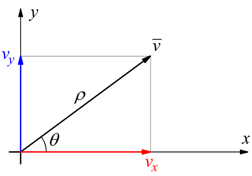
\includegraphics[width=8cm]{piano_cartesiano.png}
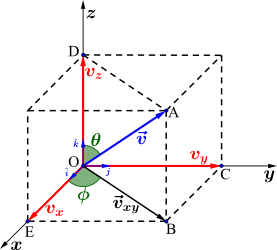
\includegraphics[width=6cm]{piano_tre_dimensioni.png}
\\
\subsubsection{Dimensione e vettori base di uno spazio}
La dimensione di uno spazio vettoriale si definisce come il numero minimo di vettori linearmente indipendenti l'uno con l'altro necessari per necessari per creare quello spazio:
\\ Peril piano cartesiano i due vettori linearmente indipendeti sono: $\vec{j}(1,0) e \vec{i}(0,1) $
\\ Per il piano a tre dimensioni: $ \vec{j}(1,0,0), \vec{i}(0,1,0), \vec{k}(0,0,1) $
\\ Questi vettori sono chiamati vettori base.
\\Due vettori sono linearmente indipendeti se la loro combinazione lineare vale 0 se e solo se i coefficienti che moltiplicano i vettori sono nulli:
$\vec{v_{1}}$ e $\vec{v_{2}} $ sono linearmente indipendenti alllora $\alpha\vec{v_{1}}*\beta\vec{v_{2}}=0$ solo per $\alpha=\beta=0 $.
\\ un esempio sono i vettori (2,3,5) e (3,7,8) \\
\[\begin{cases}
2\alpha + 3\beta=0\\
3\alpha + 7\beta=0\\
5\alpha + 8\beta=0
\end{cases}
\]
Unica soluzione $\alpha=\beta=0$ e quindi i due vettori sono linearmente indipendeti.
\\
\subsection{Spazi e matrici}
Gli spazi vettoriali possono essere definiti anche con le matrici.
\\ Infatti i vettori base possono essere scritti come matrici.
\\ prendiamo come esempio lo spazio a 4 dimensioni:
\\ un qualsiasi vettore $\vec{v}(1,2,3,4)$ può essere scritto come la somma dei vettori linearmente indipendenti:
\begin{quote} \centering (1,2,3,4)=1(1,0,0,0)+2(0,1,0,0)+3(0,0,1,0)+4(0,0,0,1)
\end{quote}
Oppure lo stesso vettore può essere scritto come matrice e come la somma delle matrici linearmenti indipendeti che compongono lo spazio:
\\
\begin{quote} \centering $\vec{v}
=\left[\begin{matrix}1& 2\\ 3 & 4\end{matrix}\right]
= 1*\left[\begin{matrix}1& 0 \\ 0 & 0\end{matrix}\right]
+ 2*\left[\begin{matrix}0 & 1 \\ 0 & 0\end{matrix}\right]
+ 3*\left[\begin{matrix}0 & 0 \\ 1 & 0\end{matrix}\right]
+ 4*\left[\begin{matrix}0 & 0 \\ 0 & 1\end{matrix}\right]
$\end{quote}
 	
\subsection{Operatore lineare}
Un operatore lineare, o trasformazione lineare, è una funzione che associa due spazi nello stesso campo, cioè una funzione che conserva l'operazione di somma di vettori e di moltiplicazione per uno scalare.
\\ Perciò se T è un operatore lineare:
\begin{quote} \centering T: $\vec{v} 
$
\begin{large} $\rightarrow$ \end{large} 
$ \vec{u}
$\end{quote}
questo vale solo se valgono le seguenti prorpietà:
\begin{itemize}
\item Additività
\begin{quote} \centering $T(\vec{v_{1}} + \vec{v_{2}})= T(\vec{v_{1}})+T(\vec{v{2}}) 
$\end{quote}
\item Omogeneità
\begin{quote} \centering $T(\alpha v)=\alpha T(v) $
\end{quote}
\end{itemize}

\subsubsection{Trasformazioni con matrici quadrate}
Se la trasformazione porta uno spazio in se stesso, l'operatore sarà una matrice quadrata.
\\ $T:R^n$
\begin{large} $\rightarrow$ \end{large} 
$R^n$
allora T sarà una matrice quadrata.
\\Riportiamo un esempio:
\\Consideriamo lo spazio vettoriale: V= $\left[\begin{matrix}a& b\\ c & d\end{matrix}\right]
$
\\ l'operatore $T: V$ \begin{large} $\rightarrow$ \end{large} $V$
\\ la matrice $M= \left[\begin{matrix}1& 2 \\ 3 & 4\end{matrix}\right]
$
\\ $A$\begin{large} $\rightarrow$ \end{large} $T(A) = MA$
\\ studio come si modificano le matrici base che chiamo $E_{1} (1,0,0,0) E_{2} (0,1,0,0) E_{3} (0,0,1,0) E_{4} (0,0,0,1)$
\\
\begin{quote} \centering $T(E_{1})= E_{1} *M= \left[\begin{matrix}1& 0\\ 0 & 0\end{matrix}\right]\left[\begin{matrix}1& 2 \\ 3 & 4\end{matrix}\right]= \left[\begin{matrix}1& 0 \\ 3 & 0\end{matrix}\right]= 1E_{1}+3E_{3}
$
\bigskip \\ $T(E_{2})= E_{2} *M= \left[\begin{matrix}0& 1\\ 0 & 0\end{matrix}\right]\left[\begin{matrix}1& 2 \\ 3 & 4\end{matrix}\right]= \left[\begin{matrix}0& 1 \\ 0 & 3\end{matrix}\right]= 1E_{2}+3E_{4}
$
\bigskip \\ $T(E_{3})= E_{3} *M= \left[\begin{matrix}0& 0\\ 1 & 0\end{matrix}\right]\left[\begin{matrix}1& 2 \\ 3 & 4\end{matrix}\right]= \left[\begin{matrix}2& 0 \\ 4 & 0\end{matrix}\right]= 2E_{1}+4E_{3}
$
\bigskip \\ $T(E_{4})= E_{4} *M= \left[\begin{matrix}0& 0\\ 0 & 1\end{matrix}\right]\left[\begin{matrix}1& 2 \\ 3 & 4\end{matrix}\right]= \left[\begin{matrix}0& 2\\ 0 & 4\end{matrix}\right]= 2E_{2}+4E_{4}
$\end{quote}
Perciò posso determinare 
\begin{quote} \centering $[T]=\left[\begin{matrix}1& 0&2&0\\ 0 & 1& 0 & 2\\3&0&4&0\\0&3&0&4\end{matrix}\right]
$ \end{quote}
Ultima osservazione che faccio è che se lo spazio iniziale è un 2*2 l'operatore lineare sarà una matrice di un ordine superione in questo caso 4.

\section{Rotazioni e numeri complessi}
In quest'ultima sezione analizziamo come le rotazioni nel piano cartesiano e i numeri complessi sono legati.
\subsection{Rotazioni nel piano cartesiano}
La rotazione in due dimensione può essere considerata una trasformazione lineare e perciò può essere rappresentata con un operatore lineare.
\\ La matrice in questione è: 
\begin{quote} \centering $\left[\begin{matrix}\cos\theta & -\sin\theta\\ \sin\theta & \cos\theta\end{matrix}\right]
$\end{quote}
\subsubsection{Esempio}
Cosideriamo il punto $P(x,y)= x(1,0)+y(0,1)$
\\ i vettori base nelle rotazioni di angolo theta si trasformano: 
\begin{quote} \centering (1,0) \begin{large} $\rightarrow$ \end{large} $(\cos\theta, \sin\theta)
$ \\
(0,1) \begin{large} $\rightarrow$ \end{large} $(-\sin\theta, \cos\theta)
$ \end{quote}
Il trasformato di P diventa:
\begin{quote} \centering $T(P)=T(x,y)=x(\cos\theta,\sin\theta)+y(-\sin\theta,\cos\theta)= (x\cos\theta-y\sin\theta,x\sin\theta+y\cos\theta)
$\end{quote}
Si ottiene lo stesso risultato considerando l'operatore lineare e il punto P come matrice:
\begin{quote} \centering $T(P)= M*P=\left[\begin{matrix}\cos\theta & -\sin\theta\\ \sin\theta & \cos\theta\end{matrix}\right]\left[\begin{matrix}x\\ y\end{matrix}\right]=(x\cos\theta-y\sin\theta,x\sin\theta+y\cos\theta)
$\end{quote}
\subsubsection{Isometria}
La trasformazione è isometrica e si può verificarlo calcolando il determinante dell'operatore:
\begin{quote} \centering Determinante$\left[\begin{matrix}\cos\theta & -\sin\theta\\ \sin\theta & \cos\theta\end{matrix}\right]= (\cos\theta)(\cos\theta)-(-\sin\theta)(\sin\theta)= \cos^2\theta+\sin^2\theta=1
$\end{quote}
Tutte le trasformazioni che presentano il determinante uguale a uno conservano le misure.
\subsection{Numeri complessi}
Ogni rotazione può essere pensata come un numero complesso. In partricolare ogni rotazione risulta il prodotto di un numero complesso di modulo 1 con un altro numero complesso (che corrisponde al punto).
\subsubsection{Verifica}
Consideriamo un numero complesso u definito:
\begin{quote} \centering $u=\cos\theta+\textit{i}\sin\theta
$\end{quote}
verifichiamo che il modulo di u=1
\begin{quote} \centering$ |u|=\sqrt{\cos^2\theta+\sin^2\theta}=1
$\end{quote}
Ora prendiamo un altro numero complesso v:
\begin{quote} \centering$v=x+\textit{i}y 
$\end{quote}
Calcoliamo il prodotto:
\begin{quote} \centering$uv=(\cos\theta+\textit{i}\sin\theta)(x+\textit{i}y)=(x\cos\theta-y\sin\theta)+\textit{i}(x\sin\theta+y\cos\theta)
$\end{quote}
Il risultato è ciò che si ottiene con le rotazioni.
\subsubsection{numeri complessi e matrici}
Proviamo a relazionare i numeri complessi e le matrici.
\\Prendiamo il numero u precedente:
\begin{quote} \centering$u=1*\cos\theta+\textit{i}\sin\theta
$\end{quote}
Scriviamo 1 come la matrice unitaria e associamo a \textit{i} un matrice, la caratteristica di quest'ultima matrice è che se elevata al quadrato il risultato è meno la matrice unitaria:
\\Infatti:
\begin{quote} \centering $\textit{i}^2=-1
$\end{quote}
Verifico che questa matrice è:
\begin{quote} \centering $\left[\begin{matrix}0&-1\\ 1&0 \end{matrix}\right]
$
\bigskip \\
$\left[\begin{matrix}0&-1\\ 1&0 \end{matrix}\right]
\left[\begin{matrix}0&-1\\ 1&0 \end{matrix}\right]
= \left[\begin{matrix}-1&0 \\ 0&-1 \end{matrix}\right]
=-\left[\begin{matrix}1&0 \\ 0&1 \end{matrix}\right]
$\end{quote}
Il numero u perciò diventa:
\begin{quote} \centering$u=\cos\theta\left[\begin{matrix}1&0 \\ 0&1 \end{matrix}\right]+\sin\theta\left[\begin{matrix}0&-1\\ 1&0 \end{matrix}\right]
$\end{quote}
Perciò un nuemero complesso può essere scritto in generale nella forma:
\begin{quote} \centering $a+b\sqrt{-1}=a \left[\begin{matrix}1&0 \\ 0&1 \end{matrix}\right]+ b\left[\begin{matrix}0&-1\\ 1&0 \end{matrix}\right]
$\end{quote}
\subsection{Rotazioni e matrici}
Allora possiamo concludere che una matrice di ordine due descrive le rotazioni nel paino cartesiano.
\section{Conclusioni}
Nelle conslusioni consideriamo un spazio vettoriale $R^4$ descritto da quattro matrici base.
\\Questo campo ragglio dei vettori chiamati quaternioni. I quaternioni furono un invenzione di un matematico inglese, Hamilton. In particolare un quaternione puro è in grado di descrivere una rotazione nello spazio $R^3$, come un numero immaginario descrive una rotazione nello spazio $R^2$.Per questa ragione i quaternioni vennero sfruttati da Wolfgang Pauli per descrivere i vettori di spin e formulare il suo principio di esclusione.
\\
Le matrici di Pauli sono:
\begin{quote} \centering$\sigma_{x}=\left[\begin{matrix}0&1\\ 1&0 \end{matrix}\right] \sigma_{y}=\left[\begin{matrix}0&-\textit{i}\\ \textit{i}&0 \end{matrix}\right] \sigma_{z}=\left[\begin{matrix}1&0\\ 0&-1 \end{matrix}\right]
$\end{quote}

\section{Bibliografia e sitografia}
- Frank Ayres Jr., Teoria ed applicazioni delle Matrici, collana Schaum, 1974\\
- Definizione operatore: https://bit.ly/2N5RAES 27/06/2018\\
- Immagine piano cartesiano: https://bit.ly/2tyzkMm 27/06/2018\\
- Immagine piano tridimensionale: https://bit.ly/2Kt8cFf 27/06/2018

\end{document}	